%\section{Theory}
\section {Early Evidence of the Internal Structure of Nucleon}
\pdfcomment{magnetic moment of proton and neutron}
The first evident of nucleons being a composite particles comes form the 
measurement of their magnetic moment. For spin 1/2 elementary particles, the 
magnetic moment can be expressed as 
\begin{equation}
\mu = \frac{g}{2}\mu_B ~~~~ \mu_B = \frac{e\hbar}{2m},
\end{equation}
with $g$ expected to be $2$. Such measurement was first carried out by Otto 
Stern in 1933. And they found that the $g$ factor for proton is significantly 
greater than $2$. Since the neutron is a neutral particle, it was expected that
to have a zero magnetic moment. Stern and his team would later found that the 
neutron moment to be non-zero, suggesting that proton and neutron are composite
particles.
\pdfcomment{find appropriate citation. The original paper on proton magnetic
	moment is in Germany which I can't read}

In the 1950s, the proton form factor was measured using electron proton elastic
scattering experiments\cite{hofstadter1956}. The electron-proton elastic 
scattering in the laboratory frame can be expressed in the Rosenbluth formula
\begin{equation}
\dv{\sigma}{\Omega} = \frac{\alpha^2}{4E^2 \sin^2\left(\theta/2\right)} 
	\frac{E^\prime}{E} \left( \frac{G_E^2+\tau G_M^2}{1+\tau} \cos^2 
	\frac{\theta}{2} + 2\tau G_M^2 \sin^2 \frac{\theta}{2}\right)
	\label{eq:ep_cs},
\end{equation}
where $\tau$ is given by
\begin{equation}
\tau = \frac{Q^2}{4m_p^2}.
\end{equation}
And $E$, $E^\prime$ are the initial and final energy of the scattered electron.
The electric ($G_E\left(Q^2\right)$) and magnetic ($G_M\left(Q^2\right)$) form
factors are functions of the four momentum squared of the virtual photon. At 
low-$Q^2$ limit, these form factors can be interpreted as the Fourier transforms
of the charge and magnetic moment distribution of the nucleon. The deviation of
the neutron electric form factor from zero illustrate the existence of internal
structures in nucleons. Fig.\ \ref{fig:charge} shows the extracted proton and 
neutron charge density from the electric form factor taken from Ref.\ 
\cite{miller2007}.
\begin{figure}[htbp!]
    \centering
    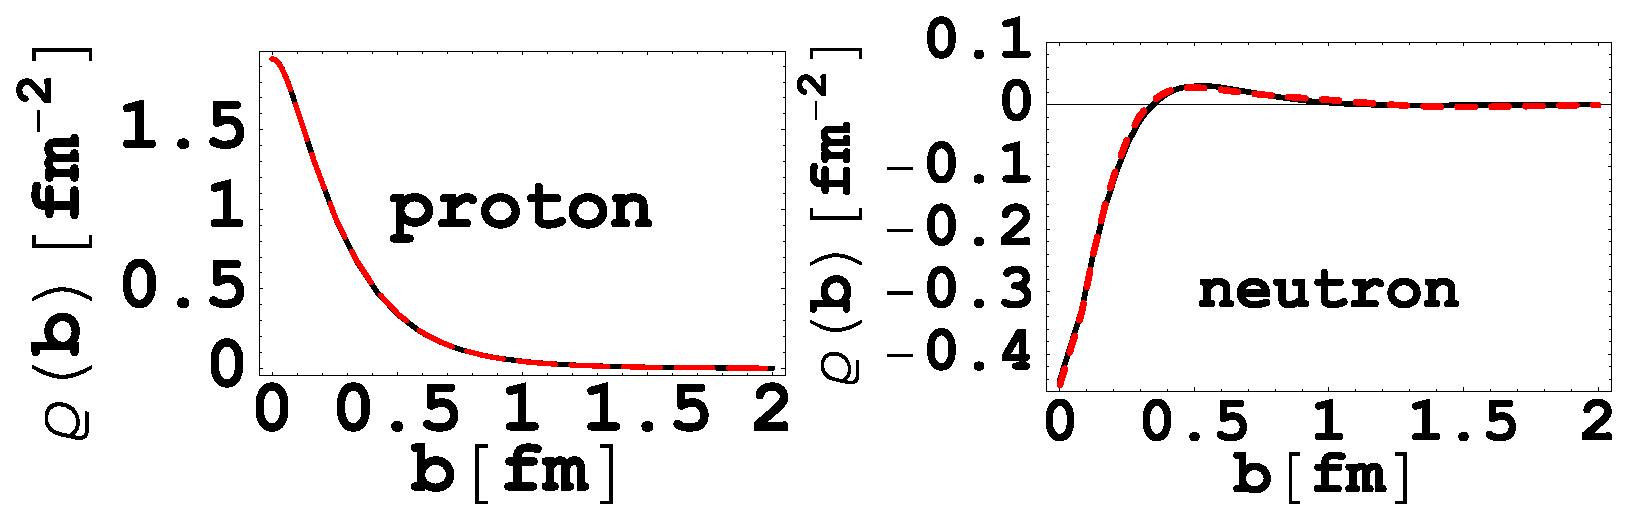
\includegraphics[width=0.9\linewidth]{./images/charge_distribution_rotated}
    \caption{The proton charge density (left panel) and neutron charge density
	(right panel). Taken from Ref.\ \cite{miller2007}}.
    \label{fig:charge}
\end{figure}


\section {Deep Inelastic Scattering}
\label{sec:dis}
Evidence of the point-like constituents in the nucleon first came from the deep
inelastic scattering (DIS) experiments \cite{breidenbach1969}, where a high 
energy lepton ($l$) is inelastically scattered of a nucleon ($N$), as 
illustrated in Fig.\ \ref{fig:DIS}
\begin{equation}
	l + N \rightarrow l^\prime + X.
\end{equation}
\begin{figure}[htbp!]
    \centering
    \includegraphics[width=0.5\linewidth]{./images/DIS}
    \caption{The Feynman diagram for DIS}
    \label{fig:DIS}
\end{figure}
Similar to Eq.\ \ref{eq:ep_cs}, the DIS cross section can be expressed as 
\begin{equation}
	\eval{\pdv{\sigma}{E^\prime}{\Omega}}_{DIS} = \frac{\alpha^2}{4E^2 \sin^4 
	\frac{\theta}{2}} \left[ W_2\left(\nu,Q^2\right)\cos^2
	\frac{\theta}{2} + W_1\left(\nu,Q^2\right)\sin^2 \frac{\theta}{2}
	\right],
	\label{eq:DIS_cs1}
\end{equation}
where $\nu$ is the energy transferred by the scattering lepton. It is also 
customary to the define the structure functions $F_{1,2}$ from $W_{1,2}$ as:
\begin{equation}
	\begin{split}
		F_1\left(x,Q^2\right) &= MW_1\left(\nu,Q^2\right)\\
		F_2\left(x,Q^2\right) &= \nu W_2\left(\nu,Q^2\right),
	\end{split}
\end{equation}
where $x=Q^2/2M\nu$ and $M$ is the mass of the nucleon. It was observed that 
these structure functions $F_{1,2}$ are independent of $Q^2$, as illustrated in
Fig.\ \ref{fig:w2}. Fig.\ \ref{fig:w2} shows the early measurements of the 
structure function $F_2=\nu W_2$ as a function of $Q^2$ for a fixed 
$x=1/\omega=0.25$ taken from Ref.\ \cite{friedman1972}. This observation is 
known as Bjorken scaling\cite{bjorken1969}.
\begin{figure}[htpb!]
	\centering
	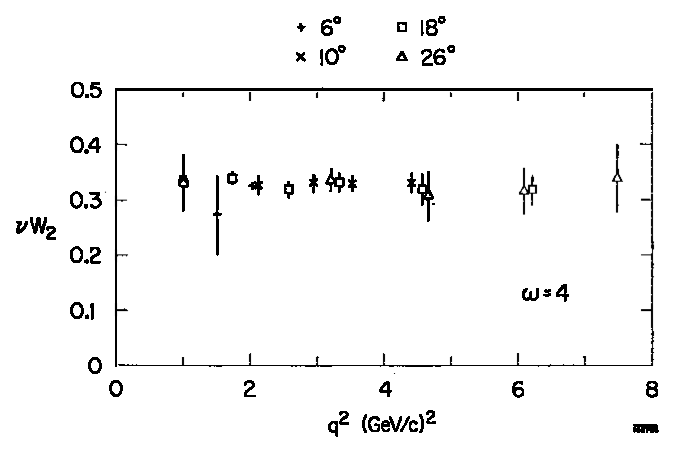
\includegraphics[width=0.5\linewidth]{images/nu_W2}
	\caption{Early measurement structure function $F_2=\nu W_2$ from 
	fixed-target electron–proton inelastic scattering at SLAC for 
	$x=1/\omega=0.25$ taken from Ref.\ \cite{friedman1972}. The observation 
	that $F_2(x,Q^2)$ is independent of $Q^2$ is known as Bjorken scaling. }
	\label{fig:w2}
\end{figure}

\section{Parton Model}
\label{sec:parton}
To explain the scaling behavior, Feynman proposed the parton model\cite{feynman1969}.
In this model,hadrons are treated as an extended objects which are made up of 
constituents (partons) held together by their mutual interaction. We now know 
these partons are quarks and gluons described by QCD, but this was not known at 
the time. In the DIS process, the high energy lepton is scattered off the 
partons elastically. In the center-of-mass frame, the hadron is Lorentz 
contracted in the direction of the collision, and the internal interaction are
time dilated. Hence as the center-of-mass energy increases, the lifetime of the
virtual partonic state is lengthened, and the time for the electron to pass 
traverse the hadron is shortened. If the lifetime of the virtual partonic states
is longer than the duration of the electron-hadron interaction, the partons are
essentially frozen and the parton-parton interactions are neglectable. One can


The ability to write the structure function and the cross section as a 
convolution of the long-range interaction and pQCD short range interaction is 
known as the factorization theorem \cite{collins1989}.


\pdfcomment{callan-gross relation shows that the protons are made up of spin 1/2
	partons. This relation would be different if the spin of partons is 
	different}
From Eq.\ \ref{eq:DIS_cs1}, it is obvious that the structure function $W_1$ is 
related to the magnetic form factor $G_E$ in Eq.\ \ref{eq:ep_cs}. 

In the case where the partons are spin 0 particles, one would expect $F_1$ to 
be zero.

The measured deviation of the Callan-Gross relation, defined as 
\begin{equation}
K_0 = \frac{F_2}{2xF_1}-1,
\end{equation}
is shown in Fig.\ \ref{fig:callan_gross}, taken from Ref.\ \cite{kendall1991}. 
For large $Q^2$, $K_0$ is consistent with zero, establishing the parton spin as
1/2.
\begin{figure}
\centering
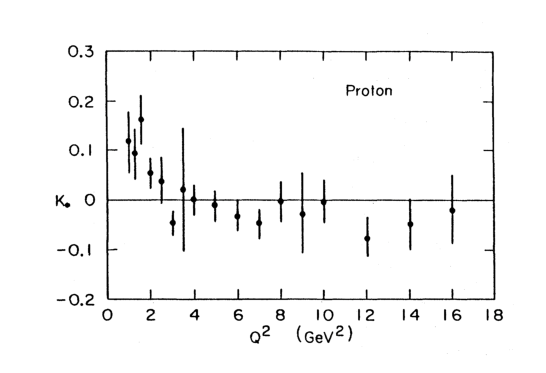
\includegraphics[width=0.5\linewidth]{images/Callan_Gross_relation}
\caption{The deviation from the Callan-Gross relation, defined as 
	$K_0=F_2/2xF_1 -1$, taken from Ref.\ \cite{kendall1991}. This result
	demonstrates the spin 1/2 nature of the partons.}
\label{fig:callan_gross}
\end{figure}


\subsection{Gottfried Sum Rule}
\label{sec:gottfried}

\section{Drell-Yan Process}
\label{sec:DY}

\pdfcomment{factorization and universality of PDF, scaling plot for both DIS 
	and DY}
\begin{figure}
\centering
\begin{subfigure}{0.45\linewidth}
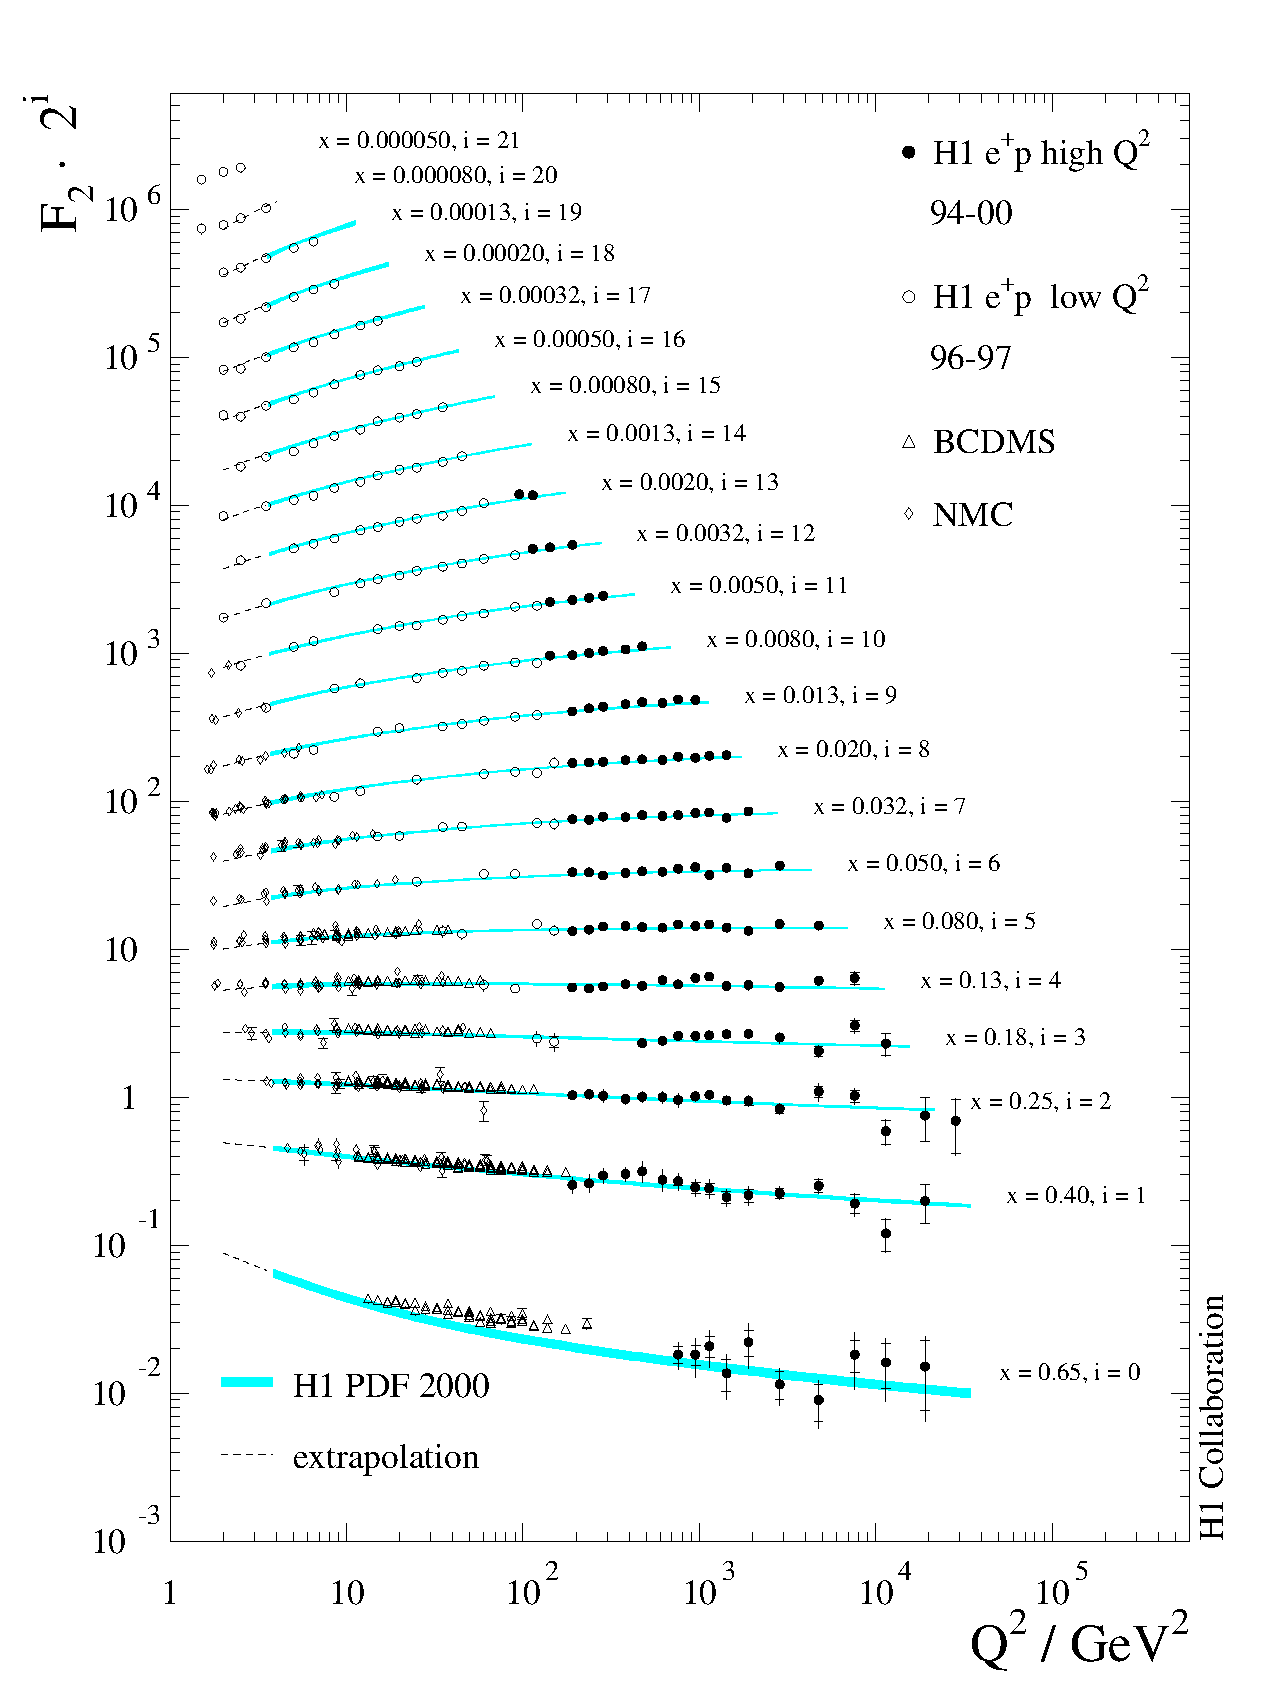
\includegraphics[width=\linewidth]{images/DIS_scaling}
\caption{taken from Ref.\ \cite{theh1collaboration2003}}
\label{subfig:DIS_scaling}
\end{subfigure}
\begin{subfigure}{0.45\linewidth}
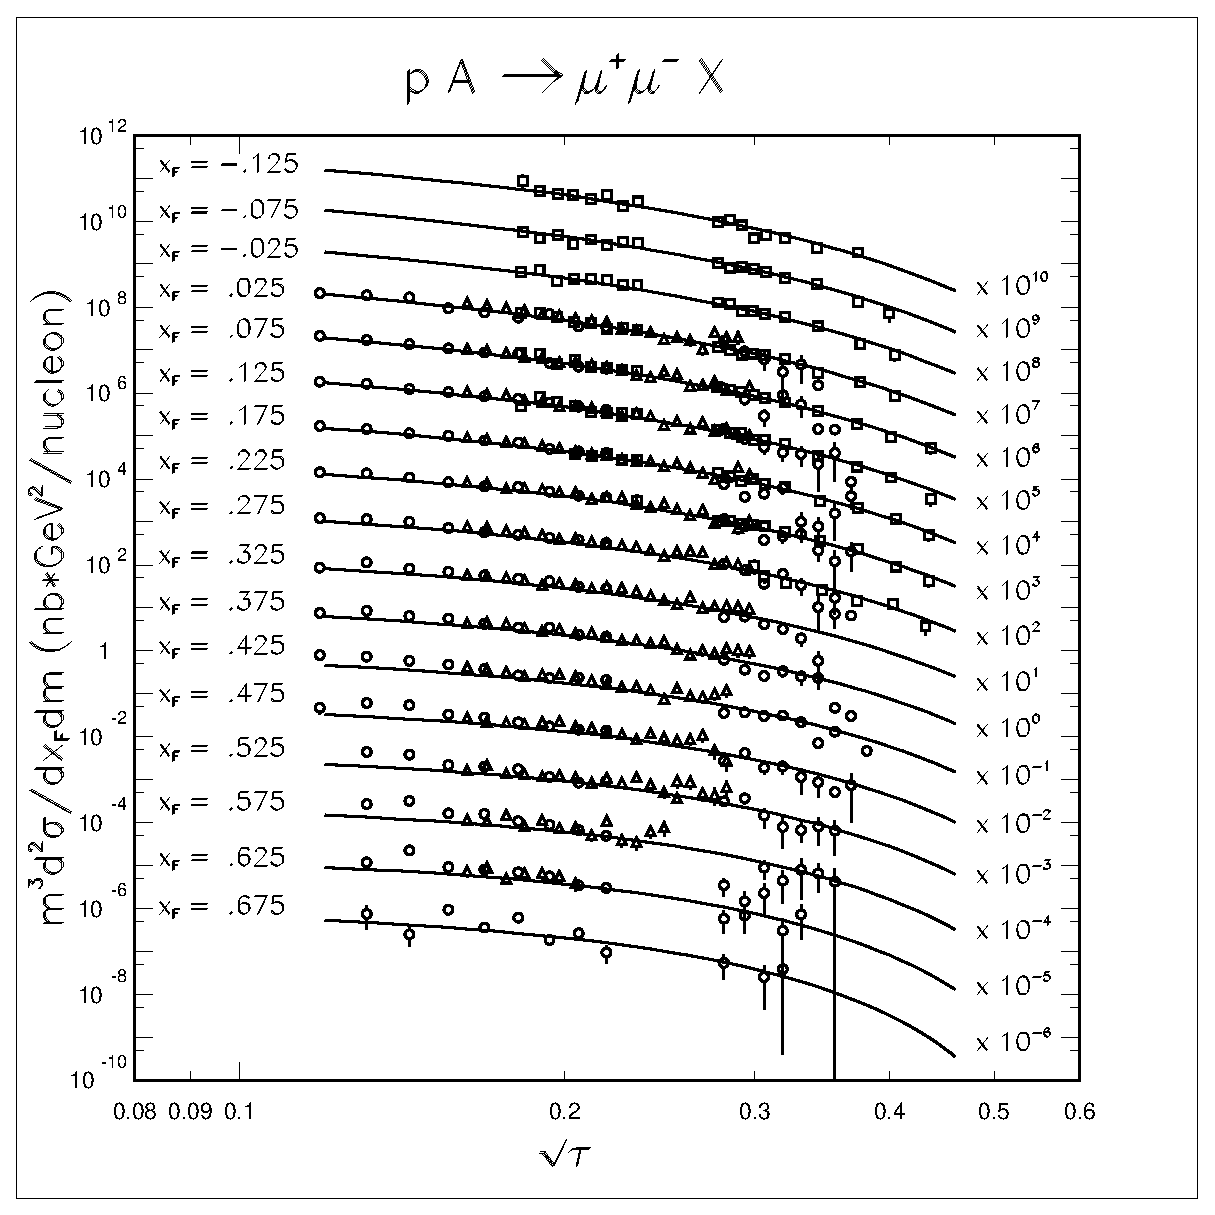
\includegraphics[width=\linewidth]{images/DY_scaling}
\caption{taken from Ref.\ \cite{mcgaughey1999}}
\label{subfig:DY_scaling}
\end{subfigure}
\caption{Compilation of data on DIS (\subref{subfig:DIS_scaling}) and Drell-Yan
 (\subref{subfig:DY_scaling})}
\end{figure}


\subsection{E866/NuSea}
\label{sec:E866}

\section{Charmonium Production}
\label{sec:jpsi}
The mechanism for charmonium production can be separated into two parts, the 
production of heavy-quark pairs and the subsequent hadronization into 
quarkonium states. One of the early approaches is the Color Evaporation method 
(CEM)\cite{einhorn1975,bodwin1995,bodwin1997}. The heavy-quark pairs production
is expanded in terms of the strong coupling constant s and is calculated with 
perturbative QCD (pQCD). CEM then assumes a constant probability $F$ for the 
$c\bar{c}$ pairs to hadronize into different charmonium state and this 
probability is independent of the kinematics or the production subprocess. The 
charmonium production cross section in the CEM framework can be expressed as
\begin{equation}
\eval{\dv{\sigma}{x_{F}}}_{J/\psi\left(\psi^\prime\right)} =
	F_{J/\psi\left(\psi^\prime\right)} \sum_{i,j=q,\bar{q},g} \int_{2m_c}^{2m_D}
\end{equation}


\pdfcomment{CEM and NRCD}

\pdfcomment{what is physical significant of the nuclear dependence}

